
\section{Causal broadcast\\for large and dynamic systems}
\label{sec:proposal}

In this section, we introduce \CBROADCAST (stands for Preventive Causal
broadcast), a causal broadcast protocol that breaks scalability barriers for
large and dynamic systems.
% It does not overload
% messages with any control information. 
To provide causal order, most
state-of-the-art~\cite{almeida2008interval,birman1987reliable,fidge1988timestamps,hadzilacos1993fault,mattern1989virtual,mostefaoui2017probabilistic,singhal1992efficient}
approaches are reactive. They check if message deliveries should be delayed to
avoid causality violations. Our approach is preventive. Messages are immediately
delivered on receipt without risk of causality violations. This difference not
only removes most of control information piggybacked in broadcast messages, but
also leads to constant delivery execution time. Protocols and applications can
finally afford causal broadcast in large and dynamic systems without loss of
efficiency.

% This section states  the definitions. It describes our algorithm. It proves that
% it handles both static and dynamic networks. It analyses its complexity.

\subsection{Model}

% Definitions and theorems come from~\cite{hadzilacos1994modular}.
A distributed system comprise processes. Processes can communicate using
messages. They may not have full knowledge of the membership, for maintenance
costs become too expansive in large and dynamic systems. Instead, processes
build overlay networks with local partial view the size of which is generally
much smaller than the actual size of the system.

\begin{definition}[Overlay network]
  An overlay network $N$ comprises a set of processes $P$. Each Process runs a
  set of instructions sequentially. \\
  An overlay network $N$ also comprises a set of links $E: P \times P$. $p$'s
  neighborhood $Q$ is the set of links departing from $p$. Processes can
  communicate with their neighbors using messages. \\
  Processes are faulty if they crash, otherwise they are correct. % The set of
  % correct processes is $C$. 
  There are no byzantine processes.
\end{definition}

For the rest of this paper, we will speak of distributed systems, overlay
networks, or networks indifferently.

\begin{definition}[Static and dynamic networks]
  A network is static if both its set of processes and its set of edges are
  immutable. Otherwise, the network is dynamic.
\end{definition}

For the rest of the paper, we only consider networks without partitions.

\begin{definition}[Network partition]
  A network has partitions if there exist two correct processes without any path
  between them, i.e., without a link or a sequence of links comprising correct
  processes only.
\end{definition}

%\TODO{Replace ``network'' by  ``distributed system'' ?}

Processes communicate by sending messages to other processes. They can send
messages to specific processes or all of them.

\begin{definition}[Uniform reliable broadcast]
  A process can broadcast a message, receive a message, and deliver a message.
  When a process broadcasts a message to all processes of the network, correct
  processes eventually receive it. 
  Uniform reliable broadcast guarantees 3 properties: \\
  \textbf{Validity:} If a correct process broadcasts a message, then it
  eventually delivers it. \\
  \textbf{Uniform Agreement:} If a process -- correct or not -- delivers a
  message, then all correct processes eventually deliver it. \\
  \textbf{Uniform Integrity:} A process delivers a message at most once, and
  only if it was previously broadcast.
\end{definition}

\begin{algorithm}[h]
  \SetKwProg{Function}{function}{}{}
\SetKwProg{Upon}{upon}{}{}
\SetKwProg{Initially}{INITIALLY:}{}{}
\SetKwProg{Dissemination}{DISSEMINATION:}{}{}

\small

\DontPrintSemicolon
\LinesNumbered

\Initially {} {
  $Q$ \tcp*{$p$'s neighborhood}
  $received \leftarrow \varnothing$ \tcp*{To detect double receipts}
}

\BlankLine

\Dissemination{}{
  
  \Function{\textsc{R-broadcast}($m$) \tcp*[f]{$b_p(m)$}} { 
    $received \leftarrow received \cup m$ \;
    \lForEach {$q \in Q$} {\textsc{sendTo}($q,\, m$)}
    \textsc{R-deliver}($m$) \tcp*{$d_p(m)$}
  }

  \BlankLine
  
  \Upon{\textsc{receive}($m$)}{
    \If {$m \not \in received$} {
      $received \leftarrow received \cup m$ \;
      \lForEach {$q \in Q$} {\textsc{sendTo}($q,\, m$) \tcp*[f]{forward}}
      \textsc{R-deliver}($m$) \tcp*{$d_p(m)$}
    }
  }
  
}


%%% Local Variables:
%%% mode: latex
%%% TeX-master: "../paper"
%%% End:

  \caption{\label{algo:reliablebroadcast}R-broadcast at Process $p$.}
\end{algorithm}

Algorithm~\ref{algo:reliablebroadcast} shows the instructions of a uniform
reliable broadcast. It uses a structure that keeps track of received messages in
order to deliver them at most once. 
%It uses a peer-sampling protocol that
%provides neighbors to communicate with, i.e., a set of links. 
%%Assuming a network without partitions meaning that there exists at least one
%path from any process to any correct process, then all correct processes
%eventually receive all messages at least once:
Since processes may not have full membership knowledge, processes must forward
broadcast messages. Since the network does not have partitions, processes either
receive the message directly from the broadcaster or transitively. Thus, all
correct processes eventually deliver all messages exactly once. R-broadcast
ensures validity, uniform agreement, and uniform integrity.

% At this point, processes receive and deliver each message exactly once. However,
% R-broadcast delivers messages in any order.  In addition to reliably conveying
% messages to all correct processes. 

Broadcast protocols can also ensure a specific ordering among message
deliveries.
%that messages are delivered in a specific order.
To define a delivery order among messages, we define time in a logical sense
using Lamport's definition~\cite{lamport1978time}.

\begin{definition}[Happen before~\cite{lamport1978time}]
  Happen before is a transitive, irreflexive, and antisymmetric relation that
  defines a strict partial orders of events.  The sending of a message always
  precedes its receipt.
\end{definition}

To order messages broadcast from one process, we define FIFO order.

\begin{definition}[FIFO order]
  If a process broadcasts a first message then broadcasts a second message,
  processes deliver the first message before the second message.
\end{definition}

To order messages broadcast by different processes, we define local order.

\begin{definition}[Local order]
  If a process broadcasts a message after having delivered another message
  broadcast by another process, processes deliver the latter before the former.
\end{definition}

To order messages broadcast by every processes, we define causal order.

\begin{definition}[Causal order]
  The delivery order of messages follows the happen before relationships of the
  corresponding broadcasts.
\end{definition}

\begin{theorem}[\label{theo:causal}Causal order equivalence~\cite{hadzilacos1994modular}]
  The conjunction of FIFO order and local order is equivalent to causal order.
\end{theorem}

\begin{definition}[Causal broadcast]
  Causal broadcast is a uniform reliable broadcast ensuring causal order.
\end{definition}

\begin{theorem}[\label{theo:flooding}Constraint flooding in deterministic
  overlay networks is causal~\cite{friedman2004causal}]
  In static networks, a broadcast protocol is causal if it uses FIFO links,
  forwards all broadcast messages exactly once, and uses all its outgoing links.
\end{theorem}

From Theorem~\ref{theo:flooding}, reliable broadcast from
Algorithm~\ref{algo:reliablebroadcast} is causal if communication links employed
to communicate with neighbors in $Q$ are FIFO. This holds only for static
networks where $Q$ is immutable. In practice, processes add and remove links to
neighbors from $Q$ at any time. Next section describes a preventive causal
broadcast that handles such dynamicity.


\subsection{Operation}

\begin{algorithm}[h]
  
\SetKwProg{Function}{function}{}{}
\SetKwProg{Upon}{upon}{}{}
\SetKwProg{Initially}{INITIALLY:}{}{}
\SetKwProg{Dissemination}{DISSEMINATION:}{}{}
\SetKwProg{Safety}{SAFETY:}{}{}

\small

\DontPrintSemicolon
\LinesNumbered

\Initially {} {
  $Q$ \tcp*{$p$'s neighborhood, FIFO channels}
  $B \leftarrow \varnothing$ \tcp*{Buffers of messages}
}

\BlankLine

\Safety {} {
  \Upon{\textsc{open}($q$)} {
    \If{$|Q|>1$} {
      $Q \leftarrow Q \setminus q$ \;
      $B[q] \leftarrow \varnothing$ \;
      $\textsc{sendLocked}(p,\, q)$ \;
    }
  }
  
  \BlankLine
  
  \Upon{\textsc{receiveLocked}($from, \, to$) \tcp*[f]{$to=p$}} {
    $\textsc{sendAck}(from,\, to)$ \;
  }
  
  \BlankLine

  \Upon{\textsc{receiveAck}($from,\, to$) \tcp*[f]{$from=p$}} {
    \If {$to \in B$} {
      \lForEach {$m \in B[to]$} {$\textsc{sendTo}(to,\, m)$}
      $B \leftarrow B \setminus to$ \;
      $Q \leftarrow Q \cup to$ \;
    }
  }

  \BlankLine

  \Upon{\textsc{close}($q$)} {
    $B \leftarrow B \setminus q$ \;
  }

}

\BlankLine

\Dissemination {} {

  \Function{\textsc{FBC-broadcast}$^+$($m$) \tcp*[f]{$b_p(m)$}} {    
    \lForEach {$q \in B$} {$B[q] \leftarrow B[q] \cup m$ \tcp*[f]{Buffers}}
    $\textsc{R-broadcast}(m)$ \;
  }
  
  \BlankLine
  
  \Upon{\textsc{R-deliver}($m$)} {
    \lForEach {$q \in B$} {$B[q] \leftarrow B[q] \cup m$ \tcp*[f]{Buffers}}
    $\textsc{FBC-deliver}^+(m)$ \tcp*{$d_p(m)$}
  }

}


%%% Local Variables:
%%% mode: latex
%%% TeX-master: "../paper"
%%% End:

  \caption{\label{algo:bufferbroadcast}\CBROADCAST at Process $p$.}
\end{algorithm}

\begin{figure*}
  \begin{center}
    \subfloat[Part A][\label{fig:preventivesolveA}Process~A broadcasts $a$.]
    {
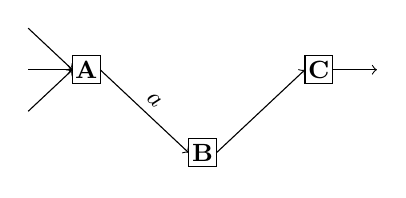
\begin{tikzpicture}[scale=1]
  
  \small
  
  \newcommand\X{210/5pt};
  \newcommand\Y{30pt};
  
  \draw[->] ( -0.5*\X, 0.5*\Y) -- ( -5+0*\X, 0*\Y);
  \draw[->] ( -0.5*\X, 0*\Y) -- ( -5+0*\X, 0*\Y);
  \draw[->] ( -0.5*\X, -0.5*\Y) -- ( -5+0*\X, 0*\Y);  

  \draw[fill=white] (0*\X, 0*\Y) node{\textbf{A}} +(-5pt, -5pt) rectangle +(5pt, 5pt);
  \draw[fill=white] (1*\X, -1*\Y) node{\textbf{B}} +(-5pt, -5pt) rectangle +(5pt, 5pt);
  \draw[fill=white] (2*\X,  0*\Y) node{\textbf{C}} +(-5pt, -5pt) rectangle +(5pt, 5pt);

  \draw[->](5+0*\X, 0*\Y) -- node[sloped, above]{$a$} (-5+1*\X, -1*\Y); %% A->B
  \draw[->](5+1*\X, -1*\Y) -- (-5+2*\X, 0*\Y); %% B->D

  \draw[->](5+2*\X, 0*\Y) -- ( 2.5*\X, 0*\Y);
\end{tikzpicture}}
    \hspace{20pt}
    \subfloat[Part B][\label{fig:preventivesolveB}Process~A wants
    to add a link to Process~D. 
    It sends a ping message $\pi$ to Process~D using one of its FIFO links.]
    {
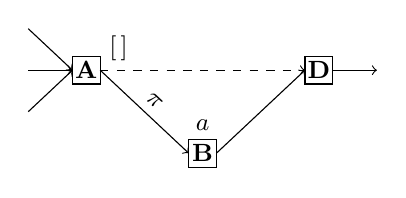
\begin{tikzpicture}[scale=1]
  
  \small
  
  \newcommand\X{210/5pt};
  \newcommand\Y{30pt};
  
  \draw[->] ( -0.5*\X, 0.5*\Y) -- ( -5+0*\X, 0*\Y);
  \draw[->] ( -0.5*\X, 0*\Y) -- ( -5+0*\X, 0*\Y);
  \draw[->] ( -0.5*\X, -0.5*\Y) -- ( -5+0*\X, 0*\Y);  

  \draw[fill=white] (0*\X, 0*\Y) node{\textbf{A}} +(-5pt, -5pt) rectangle +(5pt, 5pt);
  \draw[fill=white] (1*\X, -1*\Y) node{\textbf{B}} +(-5pt, -5pt) rectangle +(5pt, 5pt);
  \draw (1*\X, 5-1*\Y) node[anchor=south]{$a$};
  \draw[fill=white] (2*\X,  0*\Y) node{\textbf{D}} +(-5pt, -5pt) rectangle +(5pt, 5pt);

  \draw[->](5+0*\X, 0*\Y) -- node[sloped, above]{$\pi$} (-5+1*\X, -1*\Y); %% A->B
  \draw[->](5+1*\X, -1*\Y) -- (-5+2*\X, 0*\Y); %% B->D
  
  \draw[->, dashed] (5+0*\X, 0*\Y) node[anchor=south west]{$[\,]$} -- (-5+2*\X, 0*\Y); %% A->B

  \draw[->](5+2*\X, 0*\Y) -- ( 2.5*\X, 0*\Y);
\end{tikzpicture}}
    \hspace{20pt}
    \subfloat[Part C][\label{fig:preventivesolveC}Process~A broadcasts $a'$.
    It does not send it through the new link but buffers it.]
    {
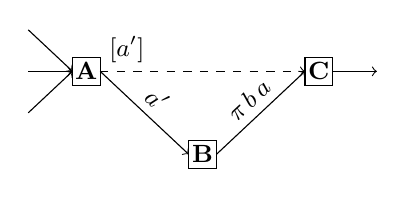
\begin{tikzpicture}[scale=1]
  
  \small
  
  \newcommand\X{210/5pt};
  \newcommand\Y{30pt};
  
  \draw[->] ( -0.5*\X, 0.5*\Y) -- ( -5+0*\X, 0*\Y);
  \draw[->] ( -0.5*\X, 0*\Y) -- ( -5+0*\X, 0*\Y);
  \draw[->] ( -0.5*\X, -0.5*\Y) -- ( -5+0*\X, 0*\Y);  

  \draw[fill=white] (0*\X, 0*\Y) node{\textbf{A}} +(-5pt, -5pt) rectangle +(5pt, 5pt);
  \draw[fill=white] (1*\X, -1*\Y) node{\textbf{B}} +(-5pt, -5pt) rectangle +(5pt, 5pt);
%  \draw (1*\X, 5-1*\Y) node[anchor=south]{$a$};
  \draw[fill=white] (2*\X,  0*\Y) node{\textbf{C}} +(-5pt, -5pt) rectangle +(5pt, 5pt);

  \draw[->](5+0*\X, 0*\Y) -- node[sloped, above]{$a'$} (-5+1*\X, -1*\Y); %% A->B
  \draw[->](5+1*\X, -1*\Y) -- node[sloped, above]{$\pi\,b\,a$} (-5+2*\X, 0*\Y); %% B->D
  
  \draw[->, dashed] (5+0*\X, 0*\Y) node[anchor=south west]{$[a']$} --  (-5+2*\X, 0*\Y); %% A->B

  \draw[->](5+2*\X, 0*\Y) -- ( 2.5*\X, 0*\Y);
\end{tikzpicture}}
    \hspace{20pt}
    \subfloat[Part D][\label{fig:preventivesolveD}Process~D receives
    $\pi$ and replies to $A$.
    The reply $\rho$ can travel by any communication
    mean.]
    {
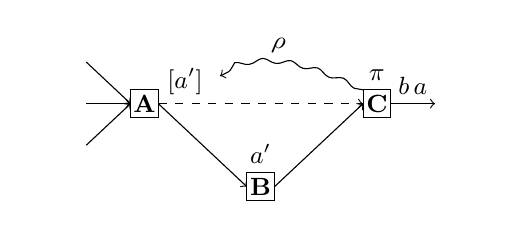
\begin{tikzpicture}[scale=1]
  
  \small
  
  \newcommand\X{210/5pt};
  \newcommand\Y{30pt};

  \draw (-1*\X, 0*\Y);
  \draw (3*\X, 0*\Y);

  
  \draw[->] ( -0.5*\X, 0.5*\Y) -- ( -5+0*\X, 0*\Y);
  \draw[->] ( -0.5*\X, 0*\Y) -- ( -5+0*\X, 0*\Y);
  \draw[->] ( -0.5*\X, -0.5*\Y) -- ( -5+0*\X, 0*\Y);  

  \draw[fill=white] (0*\X, 0*\Y) node{\textbf{A}} +(-5pt, -5pt) rectangle +(5pt, 5pt);
  \draw[fill=white] (1*\X, -1*\Y) node{\textbf{B}} +(-5pt, -5pt) rectangle +(5pt, 5pt);
  \draw (1*\X, 5-1*\Y) node[anchor=south]{$a'$};
  \draw[fill=white] (2*\X,  0*\Y) node{\textbf{C}} +(-5pt, -5pt) rectangle +(5pt, 5pt);
  \draw (2*\X, 5-0*\Y) node[anchor=south]{$\pi$};

  \draw[->](5+0*\X, 0*\Y) -- (-5+1*\X, -1*\Y); %% A->B
  \draw[->](5+1*\X, -1*\Y) -- (-5+2*\X, 0*\Y); %% B->D
  
  \draw[->, dashed] (5+0*\X, 0*\Y) node[anchor=south west]{$[a']$} --  (-5+2*\X, 0*\Y); %% A->B

  \draw[->, decorate, decoration={snake, amplitude=0.3mm}](-5+2*\X, 5+0*\Y)
  to[out=180-25, in=25] node[sloped, above left]{$\rho$}(0.65*\X, 10+0*\Y); 

  \draw[->](5+2*\X, 0*\Y) -- node[anchor=south]{$b\,a$}( 2.5*\X, 0*\Y);
\end{tikzpicture}}
    \hspace{20pt}
    \subfloat[Part E][\label{fig:preventivesolveE}Process~A receives
    Process~D's reply. 
    The former safely empties its buffer to Process~D. 
    Using the new link cannot cause causal order violation anymore.]
    {
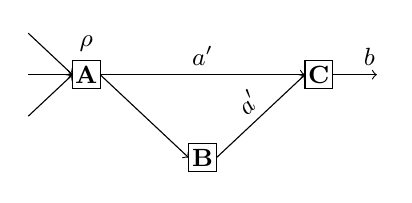
\begin{tikzpicture}[scale=1]
  
  \small
  
  \newcommand\X{210/5pt};
  \newcommand\Y{30pt};
  
  \draw[->] ( -0.5*\X, 0.5*\Y) -- ( -5+0*\X, 0*\Y);
  \draw[->] ( -0.5*\X, 0*\Y) -- ( -5+0*\X, 0*\Y);
  \draw[->] ( -0.5*\X, -0.5*\Y) -- ( -5+0*\X, 0*\Y);  

  \draw[fill=white] (0*\X, 0*\Y) node{\textbf{A}} +(-5pt, -5pt) rectangle +(5pt, 5pt);
  \draw (0*\X, 5-0*\Y) node[anchor=south]{$\rho$};
  \draw[fill=white] (1*\X, -1*\Y) node{\textbf{B}} +(-5pt, -5pt) rectangle +(5pt, 5pt);
  \draw[fill=white] (2*\X,  0*\Y) node{\textbf{C}} +(-5pt, -5pt) rectangle +(5pt, 5pt);

  \draw[->](5+0*\X, 0*\Y) -- (-5+1*\X, -1*\Y); %% A->B
  \draw[->](5+1*\X, -1*\Y) -- node[sloped, above]{$a'$} (-5+2*\X, 0*\Y); %% B->D
  
  \draw[->] (5+0*\X, 0*\Y)  -- node[anchor=south]{$a'$} (-5+2*\X, 0*\Y); %% A->B

  \draw[->](5+2*\X, 0*\Y) -- node[anchor=south west]{$b$}( 2.5*\X, 0*\Y);
\end{tikzpicture}}
    \caption{\label{fig:preventivesolve}Preventive causal broadcast does not violate
      causal order in dynamic networks anymore.}
  \end{center}
\end{figure*}

Algorithm~\ref{algo:bufferbroadcast} shows the instructions of \CBROADCAST. Its
two operations broadcast and deliver rely on reliable broadcast (see
Algorithm~\ref{algo:reliablebroadcast}). In fact, without additions nor removals
of links, our protocol only executes instructions of reliable broadcast (see
Line~\ref{line:rbroadcast},~\ref{line:rdeliver}).

\begin{theorem}[\CBROADCAST is causal in static networks\label{theo:static}]
  \CBROADCAST is a causal broadcast in static networks.
\end{theorem}

\begin{proof}
  In static networks, \CBROADCAST only executes the instructions of reliable
  broadcast. Reliable broadcast along with FIFO links ensures causal broadcast.
  The proof can be found in~\cite{friedman2004causal}.
\end{proof}

The removal of links and the departure of processes are not an issue, for it
does not reorder messages traveling through the links\footnote{It may create
  partitions infringing the uniform agreement property. Network partitioning
  constitutes an orthogonal problem that we do not address in this
  paper.}. Algorithm~\ref{algo:bufferbroadcast} does not provide specific
instructions for such cases.
% However, it may create partitions. It is an orthogonal problem

\begin{lemma}[\CBROADCAST is causal in dynamic networks subject to
  removals\label{lem:removals}]
  \CBROADCAST is a causal broadcast in dynamic networks where processes can
  leave the network or links can be removed.
\end{lemma}

\begin{proof}
  Removing a process from the network and removing all the incoming and outgoing
  links of this process is equivalent. We assume that removals do not create
  network partitions.  Removing a link does not change the delivery order of
  causally related messages. Identically to the proof of
  Theorem~\ref{theo:static}, our causal broadcast only executes instructions of
  reliable broadcast in such cases. The proof can be found
  in~\cite{friedman2004causal}.
\end{proof}

% Our causal broadcast becomes more sophisticated when the process adds links.
Unfortunately, adding links may infringe the causal order property of causal
broadcast.  Figure~\ref{fig:preventiveproblem} shows the issue with link
additions.  New links may act as shortcut for messages. First messages that
travel through new links may arrive before preceding messages that took longer
paths.
% New links create additional diffusion paths that potentially disorder
% messages.

To solve this issue, we define the safety of a link. \CBROADCAST uses all and
only safe links to disseminate messages.

% To solve this issue, we mark new links as \emph{unsafe}, for it may lead to
% causal order violations. A link becomes \emph{safe} once it conveyed all
% broadcast messages in causal order.

\begin{definition}[Safe link]
  % A link is safe if it cannot cause causal order violation.  
  A link from Process~A to Process~B is safe if and only if Process~B delivered
  or will deliver all messages delivered by Process~A before receiving any
  message that Process~A will deliver.
  % A delivered messages that
  % \begin{itemize}
  % \item B delivered, or
  % \item B will deliver
  % \end{itemize} 
  % before B receives any message that A will deliver: \\
  $safe(AB) \equiv \forall m,\, m',\, d_A(m) \rightarrow s_{AB}(m') \implies
  d_B(m) \rightarrow r_{AB}(m')$
\end{definition}

Added links start unsafe. In Figure~\ref{fig:preventiveproblem}, Process~A uses
the link to broadcast $a'$ while it is unsafe: Process~B did not deliver $a$
yet, and there was no guaranty that Process~B would deliver $a$ before receiving
$a'$ from the new link. In this example, the worst happens and Process~B
receives then delivers $a'$ before $a$ which violates causal order.

The challenge is to make unsafe links safe using local knowledge only. A
straightforward mean for Process~A to achieve this consists in sending all its
delivered messages to Process~B using this unsafe link. This guarantees that any
message delivered by A will be delivered by B before A starts using the new --
now safe -- link for causal broadcast. However, this is costly both in local
space and generated traffic.

Instead of sending all its delivered messages, Process~A builds an array of
messages to send. It makes sure that all messages it delivered that are not in
the array are already delivered by Process~B. Using safe links, Process~A sends
a signal to Process~B and awaits for a reply. While awaiting, Process~A records
all messages it delivers in the array to send. Once Process~A gets the reply, it
knows that all messages it delivered before the signal are delivered by
Process~B. Then, Process~A guarantees the receipt by B of messages it delivered
later by sending the array of messages using the unsafe link. The link becomes
safe.

% % Solving this issue requires that even new links convey all messages in the right
% %order.
% Sending all broadcast messages since the beginning of the system would be too
% expensive. Instead, Process~A creating a link to Process~B needs to know the
% messages received by Process~B. These are all messages that the new link does
% not need to convey.
% %to send potentially missing messages in causal order using this link.
% Using a reactive approach, obtaining Process~B's missing messages would require
% the transmission of messages the size of which is linear with the number of
% processes in the network. Using a preventive approach, it only requires to ping
% Process~B using already safe links. Once Process~A receives Process~B's reply,
% it knows that Process~B received all its broadcast and forwarded messages prior
% to the ping. Most importantly, Process~A knows that Process~B potentially misses
% messages broadcast or forwarded after this ping.  To avoid any causal order
% violation, Process~A sends the potentially missing messages to Process~B using
% the new link. The link becomes safe, for it cannot break causal order
% anymore. Process~A starts to use it normally for causal broadcast.


% would be costly in general settings, using already created FIFO links keeps it
% cheap. Once missing messages have been sent through this new link, $p$ starts to
% use it normally. New links do not create diffusion paths that could break causal
% order.

Compared to reliable broadcast, Algorithm~\ref{algo:bufferbroadcast} adds a
structure associating each new unsafe link with a buffer of
messages. Figure~\ref{fig:preventivesolve} shows how it solves causal order
violations. In Figure~\ref{fig:preventivesolveA}, Process~A broadcasts $a$.  In
Figure~\ref{fig:preventivesolveB}, it wants to add a link to Process~D. It sends
a ping message $\pi$ to process~D (see Line~\ref{line:sendlocked}) and awaits
for the latter's reply.  We leave aside the implementation of this send function
(e.g. broadcast or routing). % Although, using already safe links constitutes a
%cheap way to achieve it.
While awaiting, Process~A keeps its normal functioning and maintain a buffer of
messages associated with the unsafe link (see
Line~\ref{line:bufferbroadcast},~\ref{line:bufferforward}). In
Figure~\ref{fig:preventivesolveC}, Process~A broadcasts another message $a'$. It
sends it normally to Process~B but does not send it to Process~D
directly. Instead, it buffers it. In Figure~\ref{fig:preventivesolveD},
Process~D receives Process~A's ping message $\pi$. Since links are FIFO, it
implicitly means that Process~D also received $a$. Process~D sends a reply
$\rho$ to Process~A (see Line~\ref{line:sendack}). $\rho$ can travel through any
communication mean. In Figure~\ref{fig:preventivesolveE}, Process~A receives
$\rho$. Consequently, Process~A knows that Process~D received and delivered at
least $a$ and all preceding messages. It empties the buffer of messages to
Process~D (see Line~\ref{line:emptybuffer}). Afterwards, the new link is
safe. Process~A uses the new link normally.

\begin{figure*}
  \begin{center}
    \subfloat[part A][\label{fig:bufferproblemA}Slow ping message $\pi$.]
    {
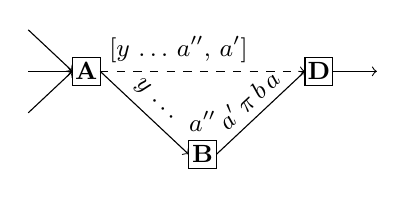
\begin{tikzpicture}[scale=1]
  
  \small
  
  \newcommand\X{210/5pt};
  \newcommand\Y{30pt};
  
  \draw[->] ( -0.5*\X, 0.5*\Y) -- ( -5+0*\X, 0*\Y);
  \draw[->] ( -0.5*\X, 0*\Y) -- ( -5+0*\X, 0*\Y);
  \draw[->] ( -0.5*\X, -0.5*\Y) -- ( -5+0*\X, 0*\Y);  

  \draw[fill=white] (0*\X, 0*\Y) node{\textbf{A}} +(-5pt, -5pt) rectangle +(5pt, 5pt);
  \draw[fill=white] (1*\X, -1*\Y) node{\textbf{B}} +(-5pt, -5pt) rectangle +(5pt, 5pt);
  \draw (1*\X, 5-1*\Y) node[anchor=south]{$a''$};
  \draw[fill=white] (2*\X,  0*\Y) node{\textbf{D}} +(-5pt, -5pt) rectangle +(5pt, 5pt);

  \draw[->, dashed] (5+0*\X, 0*\Y) -- (-5+2*\X, 0*\Y);

  \draw[->](5+0*\X, 0*\Y) node[anchor=south west]{$[y\, \ldots \,a'',\,a']$} -- node[sloped, above]{$y\, \dots$} (-5+1*\X, -1*\Y); %% A->B
  \draw[->](5+1*\X, -1*\Y) -- node[sloped, above]{$a'\,\pi\,b\,a$} (-5+2*\X, 0*\Y); %% B->D

  \draw[->](5+2*\X, 0*\Y) -- ( 2.5*\X, 0*\Y);
\end{tikzpicture}}
    \hspace{20pt}
    \subfloat[part B][\label{fig:bufferproblemB}Process~D crashes.]
    {
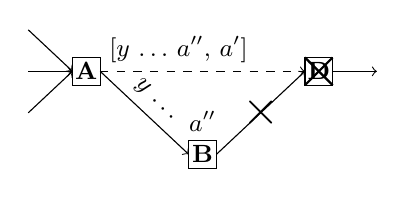
\begin{tikzpicture}[scale=1]
  
  \small
  
  \newcommand\X{210/5pt};
  \newcommand\Y{30pt};
  
  \draw[->] ( -0.5*\X, 0.5*\Y) -- ( -5+0*\X, 0*\Y);
  \draw[->] ( -0.5*\X, 0*\Y) -- ( -5+0*\X, 0*\Y);
  \draw[->] ( -0.5*\X, -0.5*\Y) -- ( -5+0*\X, 0*\Y);  

  \draw[fill=white] (0*\X, 0*\Y) node{\textbf{A}} +(-5pt, -5pt) rectangle +(5pt, 5pt);
  \draw[fill=white] (1*\X, -1*\Y) node{\textbf{B}} +(-5pt, -5pt) rectangle +(5pt, 5pt);
  \draw (1*\X, 5-1*\Y) node[anchor=south]{$a''$};
  \draw[fill=white] (2*\X,  0*\Y) node{\textbf{D}} +(-5pt, -5pt) rectangle +(5pt, 5pt);

  \draw[->, dashed] (5+0*\X, 0*\Y) -- (-5+2*\X, 0*\Y);

  \draw[->](5+0*\X, 0*\Y) node[anchor=south west]{$[y\, \ldots \,a'',\,a']$} -- node[sloped, above]{$y\,\ldots$} (-5+1*\X, -1*\Y); %% A->B
  \draw[->](5+1*\X, -1*\Y) -- % node[sloped, above]{$a'\,\ell\,b\,a$}
  node{\LARGE$\times$}(-5+2*\X, 0*\Y); %% B->D

  \draw[thick] (-5+2*\X, -5+0*\Y) -- (5+2*\X, 5+0*\Y);
  \draw[thick] (-5+2*\X, 5+0*\Y) -- (5+2*\X, -5+0*\Y);

  \draw[->](5+2*\X, 0*\Y) -- ( 2.5*\X, 0*\Y);
\end{tikzpicture}}
    \hspace{20pt}
    \subfloat[part C][\label{fig:bufferproblemC}Reply $\rho$ fails.]
    {
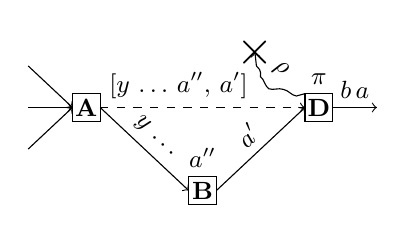
\begin{tikzpicture}[scale=1]
  
  \small
  
  \newcommand\X{210/5pt};
  \newcommand\Y{30pt};
  
  \draw[->] ( -0.5*\X, 0.5*\Y) -- ( -5+0*\X, 0*\Y);
  \draw[->] ( -0.5*\X, 0*\Y) -- ( -5+0*\X, 0*\Y);
  \draw[->] ( -0.5*\X, -0.5*\Y) -- ( -5+0*\X, 0*\Y);  

  \draw[fill=white] (0*\X, 0*\Y) node{\textbf{A}} +(-5pt, -5pt) rectangle +(5pt, 5pt);
  \draw[fill=white] (1*\X, -1*\Y) node{\textbf{B}} +(-5pt, -5pt) rectangle +(5pt, 5pt);
  \draw (1*\X, 5-1*\Y) node[anchor=south]{$a''$};
  \draw[fill=white] (2*\X,  0*\Y) node{\textbf{D}} +(-5pt, -5pt) rectangle +(5pt, 5pt);
  \draw (2*\X, 5-0*\Y) node[anchor=south]{$\pi$};

  \draw[->, dashed] (5+0*\X, 0*\Y) -- (-5+2*\X, 0*\Y);

  \draw[->](5+0*\X, 0*\Y) node[anchor=south west]{$[y\, \ldots \,a'',\,a']$} -- node[sloped, above]{$y\,\ldots$} (-5+1*\X, -1*\Y); %% A->B
  \draw[->](5+1*\X, -1*\Y) -- node[sloped, above]{$a'$} (-5+2*\X, 0*\Y); %% B->D

  \draw[->, decorate, decoration={snake, amplitude=0.3mm}](-5+2*\X, 5+0*\Y)
  to[out=180, in=-90] node[sloped, above]{$\rho$}(1.45*\X, 20+0*\Y)
  node{\LARGE$\times$}; 


  \draw[->](5+2*\X, 0*\Y) -- node[above]{$b\,a$}( 2.5*\X, 0*\Y);
\end{tikzpicture}}
    \caption{\label{fig:bufferproblem}Buffers may grow unbounded due to network
      conditions.}
  \end{center}
\end{figure*}



The ping-pong phase ensures that Process~D received all messages preceding
$a$ and $a$ itself. The buffering phase ensures that Process~D receives all
messages between the sending of the ping message $\pi$ and the receipt of
Process~D's reply $\rho$. Afterwards, Process~D will receive
Process~A's broadcast or forwarded messages from this new direct link or
transitively through Process~B.

\begin{lemma}[\CBROADCAST is causal in dynamic networks subject to
  additions\label{lem:additions}]
  \CBROADCAST is a causal broadcast in dynamic networks where processes can join
  the network or links can be added.
\end{lemma}

\begin{proof}
  To prove that \CBROADCAST is a causal broadcast, we must show that it ensures
  validity, uniform agreement, uniform integrity, and causal order. \\
  \textbf{Validity, uniform agreement, uniform integrity:} \CBROADCAST extends
  R-broadcast. Since R-broadcast ensures validity, uniform agreement, and uniform
  integrity, \CBROADCAST ensures all 3 properties. \\
  \textbf{Causal order:} From Theorem~\ref{theo:causal}, we must show
  that \CBROADCAST ensures both FIFO order and local order. \\
  \textbf{FIFO order:} Suppose a process $p$ broadcasts $m$ before
  $m'$. Consider that a correct process $q$ delivers $m'$. We must show that $q$
  delivers $m$ before $m'$. \\
  Since adding a FIFO link from a process $r$ to any other process $s$ is like
  adding potential FIFO paths from $p$ to $q$, we summarize this as a link from
  $p$ to $q$ with arbitrary settings but still FIFO.  \TODO{Should this be
    a proof?  Maybe a proof of equivalent model if kept}. \\
  Since Process $q$ delivers $m'$ it either received $m'$ from already well
  established links, or from the new one. In the former case, the proof is
  identical to that of Theorem~\ref{theo:static}. In the latter case, Process
  $q$ delivers $m'$ means that Process $p$ broadcasts $m$ then $m'$. It either
  broadcasts
  \begin{inparaenum}[(i)]
  \item \label{case:one} $m'$ during buffering and $m$ before buffering;
  \item \label{case:two} $m'$ during buffering and $m$ during buffering;
  \item \label{case:three} $m'$ after reply and $m$ before buffering;
  \item \label{case:four} $m'$ after reply and $m$ during buffering;
  \item \label{case:five} $m'$ after reply and $m$ after reply.
  \end{inparaenum}
  We must show that either 
  \begin{inparaenum}[(1)]
  \item \label{show:one} Process $q$ already received $m$ from another link
    before receiving $m'$ from the new link,
  \item \label{show:two} or that this new link conveyed $m$ before $m'$.
  \end{inparaenum}

  \begin{itemize}
  \item [(\ref{case:one})] Process $p$ put $m'$ in the buffer. Process $p$
    empties the buffer containing $m'$ after $p$ received a reply
    meaning that at least $m$ has been received at $q$. This
    shows~(\ref{show:one}).
  \item [(\ref{case:two})] Process $p$ put $m$ then $m'$ in the buffer. When the
    reply is received, it sends $m$ then $m'$ to Process $q$. This
    shows~(\ref{show:two}).
  \item [(\ref{case:three})] Identical to case~(\ref{case:one}) without the need
    of buffering.
  \item [(\ref{case:four})] Since Process $p$ empties the buffer containing $m$
    when it receives the reply, and since Process $p$ broadcasts $m'$
    afterwards using the new link, it shows~(\ref{show:two}).
  \item [(\ref{case:five})] It directly shows~(\ref{show:two}).
  \end{itemize}
  \textbf{Local order:} Since broadcast and forward have identical instructions,
  the origin of broadcast messages does not matter. The proof is identical to
  that
  of FIFO order. \\
\end{proof}

\begin{theorem}[\CBROADCAST is a causal broadcast]
  \CBROADCAST is a causal broadcast in both static and dynamic network settings.
\end{theorem}

\begin{proof}
  For static networks, it comes from Theorem~\ref{theo:static}. For dynamic
  networks, it comes from Lemmas~\ref{lem:removals}~and~\ref{lem:additions}.
\end{proof}

Algorithm~\ref{algo:bufferbroadcast} ensures causal delivery of messages even
with dynamic network settings. Compared to preventive causal broadcast for
static networks, it uses an additional local structure: buffers of messages. It
associates a buffer to each new unsafe links. We assumed that the
size of these buffer stays small in general, for it depends of the time between
the sending of ping message and the receipt of its reply which is
assumed short. However, network conditions may invalidate this
assumption. Figure~\ref{fig:bufferproblem} depicts scenarios where buffers grow
out of acceptable boundaries. In Figure~\ref{fig:bufferproblemA}, the issue
comes from high transmission delays from Process~A to Process~B, and from
Process~B to Process~D compared to the number of messages to broadcast and
forward. The ping message $\pi$ did not reach Process~D yet that the buffer
contains a lot of messages. In Figure~\ref{fig:bufferproblemB}, the issue comes
from the departure of Process~D. Depending on network settings, Process~A may
not be able to detect Process~D's departure. The former will never receive the
awaited reply and the buffer will grow forever. In
Figure~\ref{fig:bufferproblemC}, the reply $\rho$ itself fails to
reach Process~A. For the recall, this message can travel to Process~A by any
communication mean, including unreliable ones. If this fails, Process~A's buffer
to Process~D will grow forever. %as long as Process~A receives or broadcasts
%messages.

\begin{algorithm}
  
\SetKwProg{Function}{function}{}{}
\SetKwProg{Upon}{upon}{}{}
\SetKwProg{Initially}{INITIALLY:}{}{}
\SetKwProg{Dissemination}{DISSEMINATION:}{}{}
\SetKwProg{Buffer}{BOUNDING BUFFERS:}{}{}
\SetKwProg{Failure}{HANDLING FAILURES:}{}{}

\small

\DontPrintSemicolon
\LinesNumbered

\Initially {} {
  % $Q$ \tcp*{$p$'s neighborhood, FIFO channels}
  $B$ \tcp*{link $\rightarrow$ buffered messages}
  \BlankLine
  $I \leftarrow \varnothing$ \tcp*{message id $\leftrightarrow$ link}
  $R \leftarrow \varnothing$ \tcp*{link $\rightarrow$ number of retries}
  \BlankLine
  $maxSize \leftarrow \infty $ \;
  $maxRetry \leftarrow \infty$ \;
}

\BlankLine

\Buffer {} {

  \Upon{\textsc{sendLocked}($from,\, to,\, id$)}{
    \lIf{$q \not\in R$} {$R[q] \leftarrow 0$}
    $I[id] \leftarrow to$ \;
  }

  \BlankLine
  
  \Upon{\textsc{receiveAck}($from,\, to,\, id$)}{
    $I \leftarrow I \setminus id$ \;
    $R \leftarrow R \setminus to$ \;
  }
  
  \BlankLine

  \Upon{\textsc{FBC-deliver$^+$}($m$)} {
    \ForEach{$q \in B$ \textbf{\textsc{such that}} $|B[q]| > maxSize$
      \label{line:maxsize}}{
      $\textsc{retry}(q)$ \;
    }
  }

  \BlankLine

  \Upon{\textsc{close}($q$)} {
    \lFor{$i \in I$ \textbf{\textsc{such that}} $I[i]=q$}{$I \leftarrow I \setminus i$}
    $R \leftarrow R \setminus q$ \;    
  }

  \BlankLine

  \Function{\textsc{retry}($q$)}{
    \lFor{$i \in I$ \textbf{\textsc{such that}} $I[i]=q$}{$I \leftarrow I \setminus i$}
    
    \If{$q \in R$} {
      $R[q] \leftarrow R[q]+ 1$ \;
      \lIf{$R[q] \leq maxRetry$} {\textsc{open}($q$)}
      \lElse{\textsc{close}($q$)}    
    }
  }
}  

\BlankLine

\Failure {} {

  \Upon{\textsc{timeout}($from,\, to,\, id$)}{
    \lIf {$id \in I$} {\textsc{retry}($to$)\label{line:timeout}}
  }

}


%%% Local Variables:
%%% mode: latex
%%% TeX-master: "../paper"
%%% End:

  \caption{\label{algo:boundingbuffer}Bounding the size of buffers and handling
    network failures.}
\end{algorithm}

\begin{figure*}
  \begin{center}
    \subfloat[Part A][\label{fig:buffersolveA}
    Process~A wanted to add a link to Process~D after having
    broadcast $a$. Afterwards, it broadcast $a'$ and $a''$.]
    {
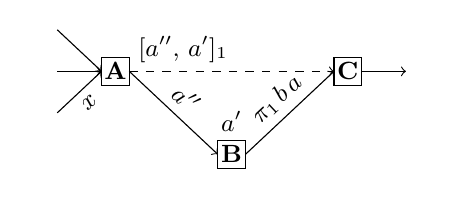
\begin{tikzpicture}[scale=1]
  
  \small
  
  \newcommand\X{210/5pt};
  \newcommand\Y{30pt};

  \draw (-0.75*\X, 0*\Y);
  \draw (2.75*\X, 0*\Y);

  
  \draw[->] ( -0.5*\X, 0.5*\Y) -- ( -5+0*\X, 0*\Y);
  \draw[->] ( -0.5*\X, 0*\Y) -- ( -5+0*\X, 0*\Y);
  \draw[->] ( -0.5*\X, -0.5*\Y) -- node[below,sloped]{$x$} ( -5+0*\X, 0*\Y);  

  \draw[fill=white] (0*\X, 0*\Y) node{\textbf{A}} +(-5pt, -5pt) rectangle +(5pt, 5pt);
  \draw[fill=white] (1*\X, -1*\Y) node{\textbf{B}} +(-5pt, -5pt) rectangle +(5pt, 5pt);
  \draw (1*\X, 5-1*\Y) node[anchor=south]{$a'$};
  \draw[fill=white] (2*\X,  0*\Y) node{\textbf{C}} +(-5pt, -5pt) rectangle +(5pt, 5pt);

  \draw[->, dashed] (5+0*\X, 0*\Y) -- (-5+2*\X, 0*\Y);

  \draw[->](5+0*\X, 0*\Y) node[anchor=south west]{$[a'',\,a']_1$} -- 
  node[sloped, above]{$a''$} (-5+1*\X, -1*\Y); %% A->B
  \draw[->](5+1*\X, -1*\Y) -- node[sloped, above]{$\pi_1\,b\,a$} (-5+2*\X, 0*\Y); %% B->D

  \draw[->](5+2*\X, 0*\Y) -- ( 2.5*\X, 0*\Y);
\end{tikzpicture}}
    \hspace{20pt}
    \subfloat[Part B][\label{fig:buffersolveB}
    Process~A receives, delivers, and forwards $x$. Since the buffer size would 
    exceed the maximal boundary, it resets the buffer with a new counter and
    sends a ping message with this counter. In the meantime, Process~D
    receives $\pi_1$ and sends the corresponding reply $\rho_1$.]
    {
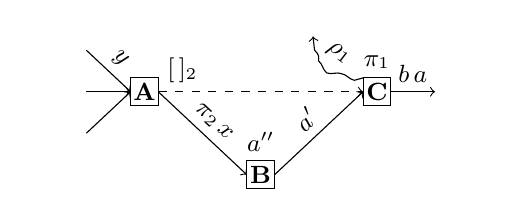
\begin{tikzpicture}[scale=1]
  
  \small
  
  \newcommand\X{210/5pt};
  \newcommand\Y{30pt};

  \draw (-1*\X, 0*\Y);
  \draw (3*\X, 0*\Y);

  
  \draw[->] ( -0.5*\X, 0.5*\Y) -- node[sloped, above]{$y$}( -5+0*\X, 0*\Y);
  \draw[->] ( -0.5*\X, 0*\Y) -- ( -5+0*\X, 0*\Y);
  \draw[->] ( -0.5*\X, -0.5*\Y) -- ( -5+0*\X, 0*\Y);  

  \draw[fill=white] (0*\X, 0*\Y) node{\textbf{A}} +(-5pt, -5pt) rectangle +(5pt, 5pt);
  \draw[fill=white] (1*\X, -1*\Y) node{\textbf{B}} +(-5pt, -5pt) rectangle +(5pt, 5pt);
  \draw (1*\X, 5-1*\Y) node[anchor=south]{$a''$};
  \draw[fill=white] (2*\X,  0*\Y) node{\textbf{C}} +(-5pt, -5pt) rectangle +(5pt, 5pt);
  \draw (2*\X, 5-0*\Y) node[anchor=south]{$\pi_1$};

  \draw[->, dashed] (5+0*\X, 0*\Y) -- (-5+2*\X, 0*\Y);

  \draw[->](5+0*\X, 0*\Y) node[anchor=south west]{$[\,]_2$} -- 
  node[sloped, above]{$\pi_2\,x$} (-5+1*\X, -1*\Y); %% A->B
  \draw[->](5+1*\X, -1*\Y) -- node[sloped, above]{$a'$} (-5+2*\X, 0*\Y); %% B->D

  \draw[->, decorate, decoration={snake, amplitude=0.3mm}](-5+2*\X, 5+0*\Y)
  to[out=180, in=-90] node[sloped, above]{$\rho_1$}(1.45*\X, 20+0*\Y);
%  node{\LARGE$\times$}; 

  \draw[->](5+2*\X, 0*\Y) -- node[above]{$b\,a$}( 2.5*\X, 0*\Y);
\end{tikzpicture}}
    \hspace{20pt}
    \subfloat[Part C][\label{fig:buffersolveC}
    Process~A forwards $y$ and buffers it. It also
    receives $\rho_1$ but no buffer exists with this counter. Process~A 
    simply discards $\rho_1$.]
    {
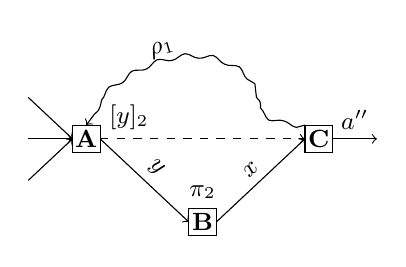
\begin{tikzpicture}[scale=1]
  
  \small
  
  \newcommand\X{210/5pt};
  \newcommand\Y{30pt};
  
  \draw[->] ( -0.5*\X, 0.5*\Y) -- ( -5+0*\X, 0*\Y);
  \draw[->] ( -0.5*\X, 0*\Y) -- ( -5+0*\X, 0*\Y);
  \draw[->] ( -0.5*\X, -0.5*\Y) -- ( -5+0*\X, 0*\Y);  

  \draw[fill=white] (0*\X, 0*\Y) node{\textbf{A}} +(-5pt, -5pt) rectangle +(5pt, 5pt);
  \draw[fill=white] (1*\X, -1*\Y) node{\textbf{B}} +(-5pt, -5pt) rectangle +(5pt, 5pt);
  \draw (1*\X, 5-1*\Y) node[anchor=south]{$\pi_2$};
  \draw[fill=white] (2*\X,  0*\Y) node{\textbf{C}} +(-5pt, -5pt) rectangle +(5pt, 5pt);
%  \draw (2*\X, 5-0*\Y) node[anchor=south]{$\ell_1$};

  \draw[->, dashed] (5+0*\X, 0*\Y) -- (-5+2*\X, 0*\Y);

  \draw[->](5+0*\X, 0*\Y) node[anchor=south west]{$[y]_2$} -- 
  node[sloped, above]{$y$}
  (-5+1*\X, -1*\Y); %% A->B
  \draw[->](5+1*\X, -1*\Y) -- node[sloped, above]{$x$} (-5+2*\X, 0*\Y); %% B->D

  \draw[decorate, decoration={snake, amplitude=0.3mm}](-5+2*\X, 5+0*\Y)
  to[out=180, in=-90] (1.45*\X, 20+0*\Y);
  \draw[->, decorate, decoration={snake, amplitude=0.3mm}](1.45*\X, 20+0*\Y)
  to[out=90+45, in=90-35] node[sloped, above]{$\rho_1$}(0*\X, 5+0*\Y);
%  node{\LARGE$\times$}; 

  \draw[->](5+2*\X, 0*\Y) -- node[above]{$a''$}( 2.5*\X, 0*\Y);
\end{tikzpicture}}
    \hspace{20pt}
    \subfloat[Part D][\label{fig:buffersolveD}
    Process~D receives $\pi_2$ and sends the corresponding
    reply $\rho_2$.]
    {
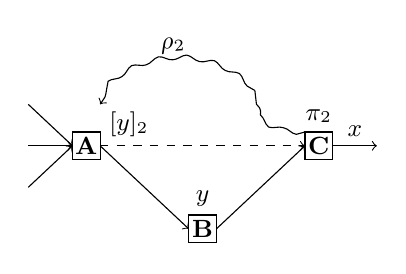
\begin{tikzpicture}[scale=1]
  
  \small
  
  \newcommand\X{210/5pt};
  \newcommand\Y{30pt};
  
  \draw[->] ( -0.5*\X, 0.5*\Y) -- ( -5+0*\X, 0*\Y);
  \draw[->] ( -0.5*\X, 0*\Y) -- ( -5+0*\X, 0*\Y);
  \draw[->] ( -0.5*\X, -0.5*\Y) -- ( -5+0*\X, 0*\Y);  

  \draw[fill=white] (0*\X, 0*\Y) node{\textbf{A}} +(-5pt, -5pt) rectangle +(5pt, 5pt);
  \draw[fill=white] (1*\X, -1*\Y) node{\textbf{B}} +(-5pt, -5pt) rectangle +(5pt, 5pt);
  \draw (1*\X, 5-1*\Y) node[anchor=south]{$y$};
  \draw[fill=white] (2*\X,  0*\Y) node{\textbf{C}} +(-5pt, -5pt) rectangle +(5pt, 5pt);
  \draw (2*\X, 5-0*\Y) node[anchor=south]{$\pi_2$};

  \draw[->, dashed] (5+0*\X, 0*\Y) -- (-5+2*\X, 0*\Y);

  \draw[->](5+0*\X, 0*\Y) node[anchor=south west]{$[y]_2$} -- 
%  node[sloped, above]{$y$}
  (-5+1*\X, -1*\Y); %% A->B
  \draw[->](5+1*\X, -1*\Y) --
  %node[sloped, above]{$a'''$}
  (-5+2*\X, 0*\Y); %% B->D

  \draw[decorate, decoration={snake, amplitude=0.3mm}](-5+2*\X, 5+0*\Y)
  to[out=180, in=-90] (1.45*\X, 20+0*\Y);
  \draw[->, decorate, decoration={snake, amplitude=0.3mm}](1.45*\X, 20+0*\Y)
  to[out=90+45, in=90-35] node[sloped, above]{$\rho_2$}(5+0*\X, 15+0*\Y);
%  node{\LARGE$\times$}; 

  \draw[->](5+2*\X, 0*\Y) -- node[above]{$x$}( 2.5*\X, 0*\Y);
\end{tikzpicture}}
    \hspace{20pt}
    \subfloat[Part E][\label{fig:buffersolveE}
    Process~A receives $\rho_2$. It empties the
    buffer with the corresponding counter. Now,  the direct link
    to Process~D is safe. Process~A uses it normally.]
    {
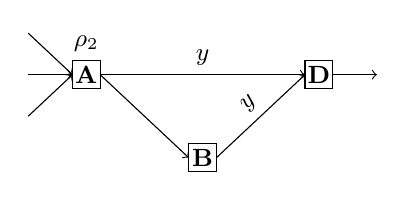
\begin{tikzpicture}[scale=1]
  
  \small
  
  \newcommand\X{210/5pt};
  \newcommand\Y{30pt};
  
  \draw[->] ( -0.5*\X, 0.5*\Y) -- ( -5+0*\X, 0*\Y);
  \draw[->] ( -0.5*\X, 0*\Y) -- ( -5+0*\X, 0*\Y);
  \draw[->] ( -0.5*\X, -0.5*\Y) -- ( -5+0*\X, 0*\Y);  

  \draw[fill=white] (0*\X, 0*\Y) node{\textbf{A}} +(-5pt, -5pt) rectangle +(5pt, 5pt);
  \draw (0*\X, 5-0*\Y) node[anchor=south]{$\rho_2$};
  \draw[fill=white] (1*\X, -1*\Y) node{\textbf{B}} +(-5pt, -5pt) rectangle +(5pt, 5pt);

  \draw[fill=white] (2*\X,  0*\Y) node{\textbf{D}} +(-5pt, -5pt) rectangle +(5pt, 5pt);
%  \draw (2*\X, 5-0*\Y) node[anchor=south]{$\ell_2$};

  \draw[->] (5+0*\X, 0*\Y) -- node[above]{$y$} (-5+2*\X, 0*\Y);

  \draw[->](5+0*\X, 0*\Y) -- (-5+1*\X, -1*\Y); %% A->B
  \draw[->](5+1*\X, -1*\Y) -- node[sloped, above]{$y$} (-5+2*\X, 0*\Y); %% B->D

  % \draw[decorate, decoration={snake, amplitude=0.3mm}](-5+2*\X, 5+0*\Y)
  % to[out=180, in=-90] (1.45*\X, 20+0*\Y);
  % \draw[->, decorate, decoration={snake, amplitude=0.3mm}](1.45*\X, 20+0*\Y)
  % to[out=90+45, in=90-35] node[sloped, above]{$\alpha_2$}(0*\X, 5+0*\Y);
%  node{\LARGE$\times$}; 

  \draw[->](5+2*\X, 0*\Y) -- ( 2.5*\X, 0*\Y);
\end{tikzpicture}}
    \caption{\label{fig:buffersolve}Buffers become bounded. We allow only 2
      elements in each buffer.}
  \end{center}
\end{figure*}

Algorithm~\ref{algo:boundingbuffer} solves the unbounded growth issue of
buffers. It solves the issue from the buffer owner's
perspective. Figure~\ref{fig:buffersolve} shows how this algorithm bounds the
size of buffers. In Figure~\ref{fig:buffersolveA}, Process~A broadcast $a$; then
wanted to add a link to Process~D so it sent a ping message; then broadcast $a'$
and $a''$ so it buffered them. We see that the ping message $\pi_1$ carries a
counter. The new buffer is identified by the same counter. In
Figure~\ref{fig:buffersolveB}, Process~A receives, delivers, and forwards the
message $x$. Each message delivery increases the size of current buffers. The
algorithm checks if the size of the buffer exceeds the configured bound (see
Line~\ref{line:maxsize}). Adding $x$ to the buffer would exceed the bound of
$2$ elements. It is first failure, so Process~A simply restarts the ping-pong
phase: it resets the buffer and sends another ping message $\pi_2$ (see
Line~\ref{line:reset}). The counter of the reset buffer is the one of the new
ping message. In the meantime, Process~D receives $\pi_1$ and sends the
corresponding reply $\rho_1$. In Figure~\ref{fig:buffersolveC}, Process~A
receives a broadcast message $y$. It delivers it, checks if the buffer can admit
it, adds the message to the buffer, and forwards it. Process~A also receives the
first reply $\rho_1$ but discards it, for no buffer has such counter. In
Figure~\ref{fig:buffersolveD}, Process~D receives $\pi_2$ and sends the
corresponding reply $\rho_2$ to Process~A. In Figure~\ref{fig:buffersolveE},
Process~A receives $\rho_2$. Since the corresponding buffer exists, it empties
it. The new link is now safe to use for causal broadcast.

While it solves the issue of unbounded buffers, it also brings another
issue. For instance, if the maximal size of buffers is too small, it could stuck
the protocol in a loop of retries. We address this issue by bounding the number
of retries. However, it means that the ping-pong phase could fail
entirely. Causal broadcast must not employ the new link. In extreme cases, it
could cause partitions in the causal broadcast overlay network. It would violate
the uniform agreement property of causal broadcast. Thus, we assume a
sufficiently large maximal bound. It never creates partitions, for most links
become safe, and the failing ones are replaced over time thanks to
network dynamicity.

Other orthogonal improvements are possible. For instance, causal broadcast could
use reliable communication means to acknowledge the receipt of the ping
message. The time taken between the sending and the receipt of the
reply would increase when failures occur. However, it would take less
time than resetting the buffering phase.

\subsection{Complexity}
\label{subsec:complexity}

We review and discuss about the complexity of \CBROADCAST. We distinguish the
complexity brought by
\begin{inparaenum}[(i)]
\item causal ordering,
\item reliable broadcast,
\item and the overlay network.
\end{inparaenum}

\PAR{Causal ordering.}{Regarding message overhead, broadcast messages convey two 
  types of control information: data to ensure FIFO order links, and
  data to globally identify the message. Thus, 
  message overhead is constant. 
  % Regarding traffic, broadcast messages do not need to convey any control
  % information. 
  Regarding number of messages, processes must send each message to all their
  neighborhood exactly once. It creates as many copies as neighbors. This number
  of copies may constitute an issue when the size of messages is large. To solve
  this issue, processes can send identifiers instead of large messages then send
  these messages on demand.  It introduces additional delays in communications
  but greatly reduces generated traffic~\cite{frey:hal-01479885}.  Regarding
  local space consumption, our protocol maintains one buffer per link during its
  ping-pong time. We assume that this time is short so the number of
  buffered messages stays small. As shown in Section~\ref{sec:proposal}, network
  conditions can make this assumption false. Algorithm~\ref{algo:boundingbuffer}
  allows to bound the size of each buffer and handle network failures.}

% While Algorithm~\ref{algo:bufferbroadcast} shows no buffer management which
% means that they can grow unbounded, we can easily bound them. For instance,
% above a threshold we clear the buffer and send another locked message, or we
% remove the link altogether.

\PAR{Reliable broadcast.}{Algorithm~\ref{algo:reliablebroadcast} shows the
  instructions of reliable broadcast. Even in presence of message duplicates it
  avoids multiple deliveries of a same message. To achieve this, the most
  straightforward structure is a set saving all new received messages. However,
  it increases linearly with the number of delivered messages (\REF). Assigning
  a unique identifier $\langle p,\, counter \rangle$ to each message changes the
  complexity. It becomes a vector that increases linearly with the number of
  processes that ever broadcast a message~\cite{fidge1988timestamps}. Using
  interval tree clocks~\cite{almeida2008interval} slightly overloads messages
  with identifiers but it improves the space complexity: the local structure
  increases linearly with the number of processes that are currently involved in
  broadcasting.}


% \TODO{Rework.} Represented in Algorithms~\ref{algo:fifobroadcast}
% and~\ref{algo:bufferbroadcast} by Function $alreadyReceived$. Causal ordering
% and detecting duplicated receipts are orthogonal problems. In this paper, we do
% not provide an implementation for the later. The simplest approach consists in
% saving all received messages (\REF). However, the size of this set linearly and
% monotonically increases as the number of broadcast messages increases. One would
% prefer an approach based on vectors where one entry corresponds to the number of
% messages received by a particular process~\cite{fidge1988timestamps}. Such
% approach do not require to piggyback additional data in the message. However, it
% requires to store locally a vector the size of which increases linearly compared
% to the number of processes that ever broadcast a message. Interval tree
% clocks~\cite{almeida2008interval} allow processes to reduce this complexity. It
% becomes linear in terms of number of processes that are currently involved in
% broadcasting. Possible improvements could take advantage of the fact that the
% number of duplicates is equal to the number of incoming links. However, it does
% not hold in dynamic networks where additional links are established. Finding a
% sublinear bound for detecting duplicated receipts remains an open problem.


\PAR{Overlay network.}{Values such as the number of messages sent by each
  process, or the number of hops for a message to reach all processes, are
  interdependent values brought by the overlay network. For instance, random
  peer-sampling protocols~\cite{jelasity2007gossip} build network overlays with
  properties similar to those of random graphs~\cite{erdos1959random}. They
  provide each process with a random subset of neighbors the size of which is
  logarithmically scaling with the network size. The number of messages sent by
  each process for each broadcast message is logarithmic.  Since random
  peer-sampling protocols build topologies close to random graphs, messages take
  a logarithmic number of hops to reach all processes. In addition, random
  peer-sampling protocols such as \SPRAY~\cite{nedelec2017adaptive} or
  \CYCLON~\cite{voulgaris2005cyclon} create links using only
  neighbor-to-neighbor interactions, i.e., they establish links only two hops
  apart. It takes only 4 hops for new links to become safe.  The overhead
  brought by these messages is negligible. The ping-pong duration,
  hence the size of buffers, remains small.}

Generated traffic remains the most important criterion for scalability. Overall,
the traffic generated by \CBROADCAST for each broadcast only depends of the size
of messages and the overlay network chosen to broadcast messages. The size of
messages is an irreducible variable; and many protocols designed to build
overlay networks achieve high scalability in terms of network size and
dynamicity (\REF). Consequently, \CBROADCAST achieve high scalability in both
these terms too. \CBROADCAST is efficient, for the upper bound on the complexity
of delivery execution time does not depend of any factor.

The next section shows an experiment that highlights the influence of
\CBROADCAST's way to ensure causal order on the underlying overlay network.

%%% Local Variables:
%%% mode: latex
%%% TeX-master: "../paper"
%%% End:
